\let\negmedspace\undefined
\let\negthickspace\undefined
\documentclass[journal]{IEEEtran}
\usepackage[a5paper, margin=10mm, onecolumn]{geometry}
\usepackage{lmodern} 
\usepackage{tfrupee} 

\setlength{\headheight}{1cm} % Set the height of the header box
\setlength{\headsep}{0mm}     % Set the distance between the header box and the top of the text

\usepackage{gvv-book}
\usepackage{gvv}
\usepackage{cite}
\usepackage{amsmath,amssymb,amsfonts,amsthm}
\usepackage{algorithmic}
\usepackage{graphicx}
\usepackage{textcomp}
\usepackage{xcolor}
\usepackage{txfonts}
\usepackage{listings}
\usepackage{enumitem}
\usepackage{mathtools}
\usepackage{gensymb}
\usepackage{comment}
\usepackage[breaklinks=true]{hyperref}
\usepackage{tkz-euclide} 
\usepackage{listings}                                      
\def\inputGnumericTable{}                                 
\usepackage[latin1]{inputenc}                                
\usepackage{color}                                            
\usepackage{array}                                            
\usepackage{longtable}
\usepackage{multicol}
\usepackage{calc}                                             
\usepackage{multirow}                                         
\usepackage{hhline}                                           
\usepackage{ifthen}                                           
\usepackage{lscape}
\begin{document}

\bibliographystyle{IEEEtran}
\vspace{3cm}

\title{5.2.34}
\author {EE25BTECH11031 - Sai Sreevallabh}
% \maketitle
% \newpage
% \bigskip
{\let\newpage\relax\maketitle}

\renewcommand{\thefigure}{\theenumi}
\renewcommand{\thetable}{\theenumi}
\setlength{\intextsep}{10pt} % Space between text and floats


\numberwithin{equation}{enumi}
\numberwithin{figure}{enumi}
\renewcommand{\thetable}{\theenumi}

\textbf{Question: }\\

Solve the given system of linear equations
\begin{center}
    $x+y=5$\\
    $2x-3y=4$\\
\end{center}

\textbf{Solution: }\\

Given lines can be represented as
\begin{align}
    \myvec{1&1}\vec{x} = 5\\
    \myvec{2&-3}\vec{x} = 4
\end{align}

Expressing the above as an augmented matrix
\begin{align}
    \augvec{2}{1}{1&1&5\\2&-3&4}
\end{align}

Converting into Reduced Row Echelon Form using row operations
\begin{align}
    \augvec{2}{1}{1&1&5\\2&-3&4} \xleftrightarrow[]{R_2 \xrightarrow{}R_2 - 2R_1} \augvec{2}{1}{1&1&5\\0&-5&-6}
\end{align}

\begin{align}
    \augvec{2}{1}{1&1&5\\0&-5&-6} \xleftrightarrow[]{R_2 \xrightarrow{}\frac{-1}{5}R_2} \augvec{2}{1}{1&1&5\\0&1&\frac{6}{5}}
\end{align}

\begin{align}
    \augvec{2}{1}{1&1&5\\0&1&\frac{6}{5}} \xleftrightarrow[]{R_1 \xrightarrow{}R_1 - R_2} \augvec{2}{1}{1&0&\frac{19}{5}\\[1ex]0&1&\frac{6}{5}}
\end{align}


\begin{align}
    \vec{x}\ =\ \myvec{\frac{19}{5}\\[1ex]\frac{6}{5}}
\end{align}

The solution of the given system of linear equations is $\myvec{\frac{19}{5}\\[1ex]\frac{6}{5}}$

\begin{figure}[h]
    \centering
    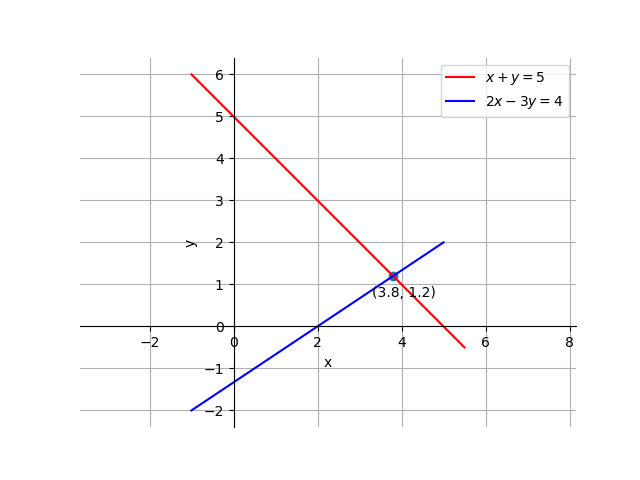
\includegraphics[width=1\columnwidth]{Figs/plot(py).png}
\end{figure}

\end{document}
